% Figure_mapping.tex — grounded OpenEarthMap(OEM) <-> Biodiversity mapping SCHEMATIC.
%
% The picture form of Table 1. Two panels + a shared legend:
%   Panel A — hard argmax (Sankey): each OEM class -> its argmax Biodiversity class, arrow
%             coloured the TARGET Biodiversity colour, confidence % on the arrow. The three
%             rows that changed from the original name-based map (Bareland -> Seminatural,
%             Water -> Grassland, Agriculture -> Grassland) are drawn with a thick black
%             outline and a grey-italic "was -> ..." annotation. Teacher-pixel-share badges
%             on the OEM chips with >3% share.
%   Panel B — soft KD transition matrix (9x6 heatmap): every cell prints P(GT student | teacher
%             OEM) x100, background = target student colour scaled by value; the per-row argmax
%             cell is bold-bordered to tie B back to A; cells <1% are blanked grey.
%
% ALL NUMBERS ARE GENERATED, NOT TRANSCRIBED:
%   scripts/figures/_gen_mapping_values.py loads artifacts/teacher_oem_gt_confusion.npz and prints
%   (a) the SOFT matrix row-normalised x100 (this is build_mapping_from_confusion(mode="B") x100),
%   (b) the per-row argmax (asserted == OEM_TO_STUDENT_PRETRAIN), and
%   (c) the teacher-pixel SHARE from the HARD array row-sums (Agriculture 66.8% etc.;
%       the SOFT array would give 63.4% for Agriculture and is NOT used for shares).
% The values embedded below are copied verbatim from that script's output (cross-checked
% against docs/FIGURE_REVISION_PLAN.md Sec 7).
%
% This is a SCHEMATIC (the value-scaled heatmap is a new schematic idiom), NOT a segmentation
% mask — do not reuse this rendering anywhere a real mask is drawn.
%
% House style (Sec 2.7): standalone + [T1]fontenc + tikz; >=Stealth; Computer Modern (no Times).
% Compile:  cd scripts/figures && pdflatex -interaction=nonstopmode -halt-on-error Figure_mapping.tex
\documentclass[border=6pt]{standalone}
\usepackage[T1]{fontenc}
\usepackage{lmodern}
\usepackage{amsmath}
\usepackage{tikz}
\usetikzlibrary{positioning, arrows.meta, calc, fit, backgrounds}

% ── Student (Biodiversity) palette — geoseg/taxonomy.py STUDENT_PALETTE ──
\definecolor{cBack}{RGB}{0,0,0}
\definecolor{cForest}{RGB}{250,62,119}
\definecolor{cGrass}{RGB}{168,232,84}
\definecolor{cCrop}{RGB}{242,180,92}
\definecolor{cSettle}{RGB}{59,141,247}
\definecolor{cSemi}{RGB}{255,214,33}

% ── OEM 8-class palette (+ Unknown black) — Figure04.py OEM8_HEX ──
\definecolor{oUnknown}{HTML}{000000}
\definecolor{oBare}{HTML}{800000}
\definecolor{oRange}{HTML}{00FF24}
\definecolor{oDev}{HTML}{949494}
\definecolor{oRoad}{HTML}{FFFFFF}
\definecolor{oTree}{HTML}{226126}
\definecolor{oWater}{HTML}{0045FF}
\definecolor{oAgri}{HTML}{4BB549}
\definecolor{oBuild}{HTML}{DE1F07}

\begin{document}
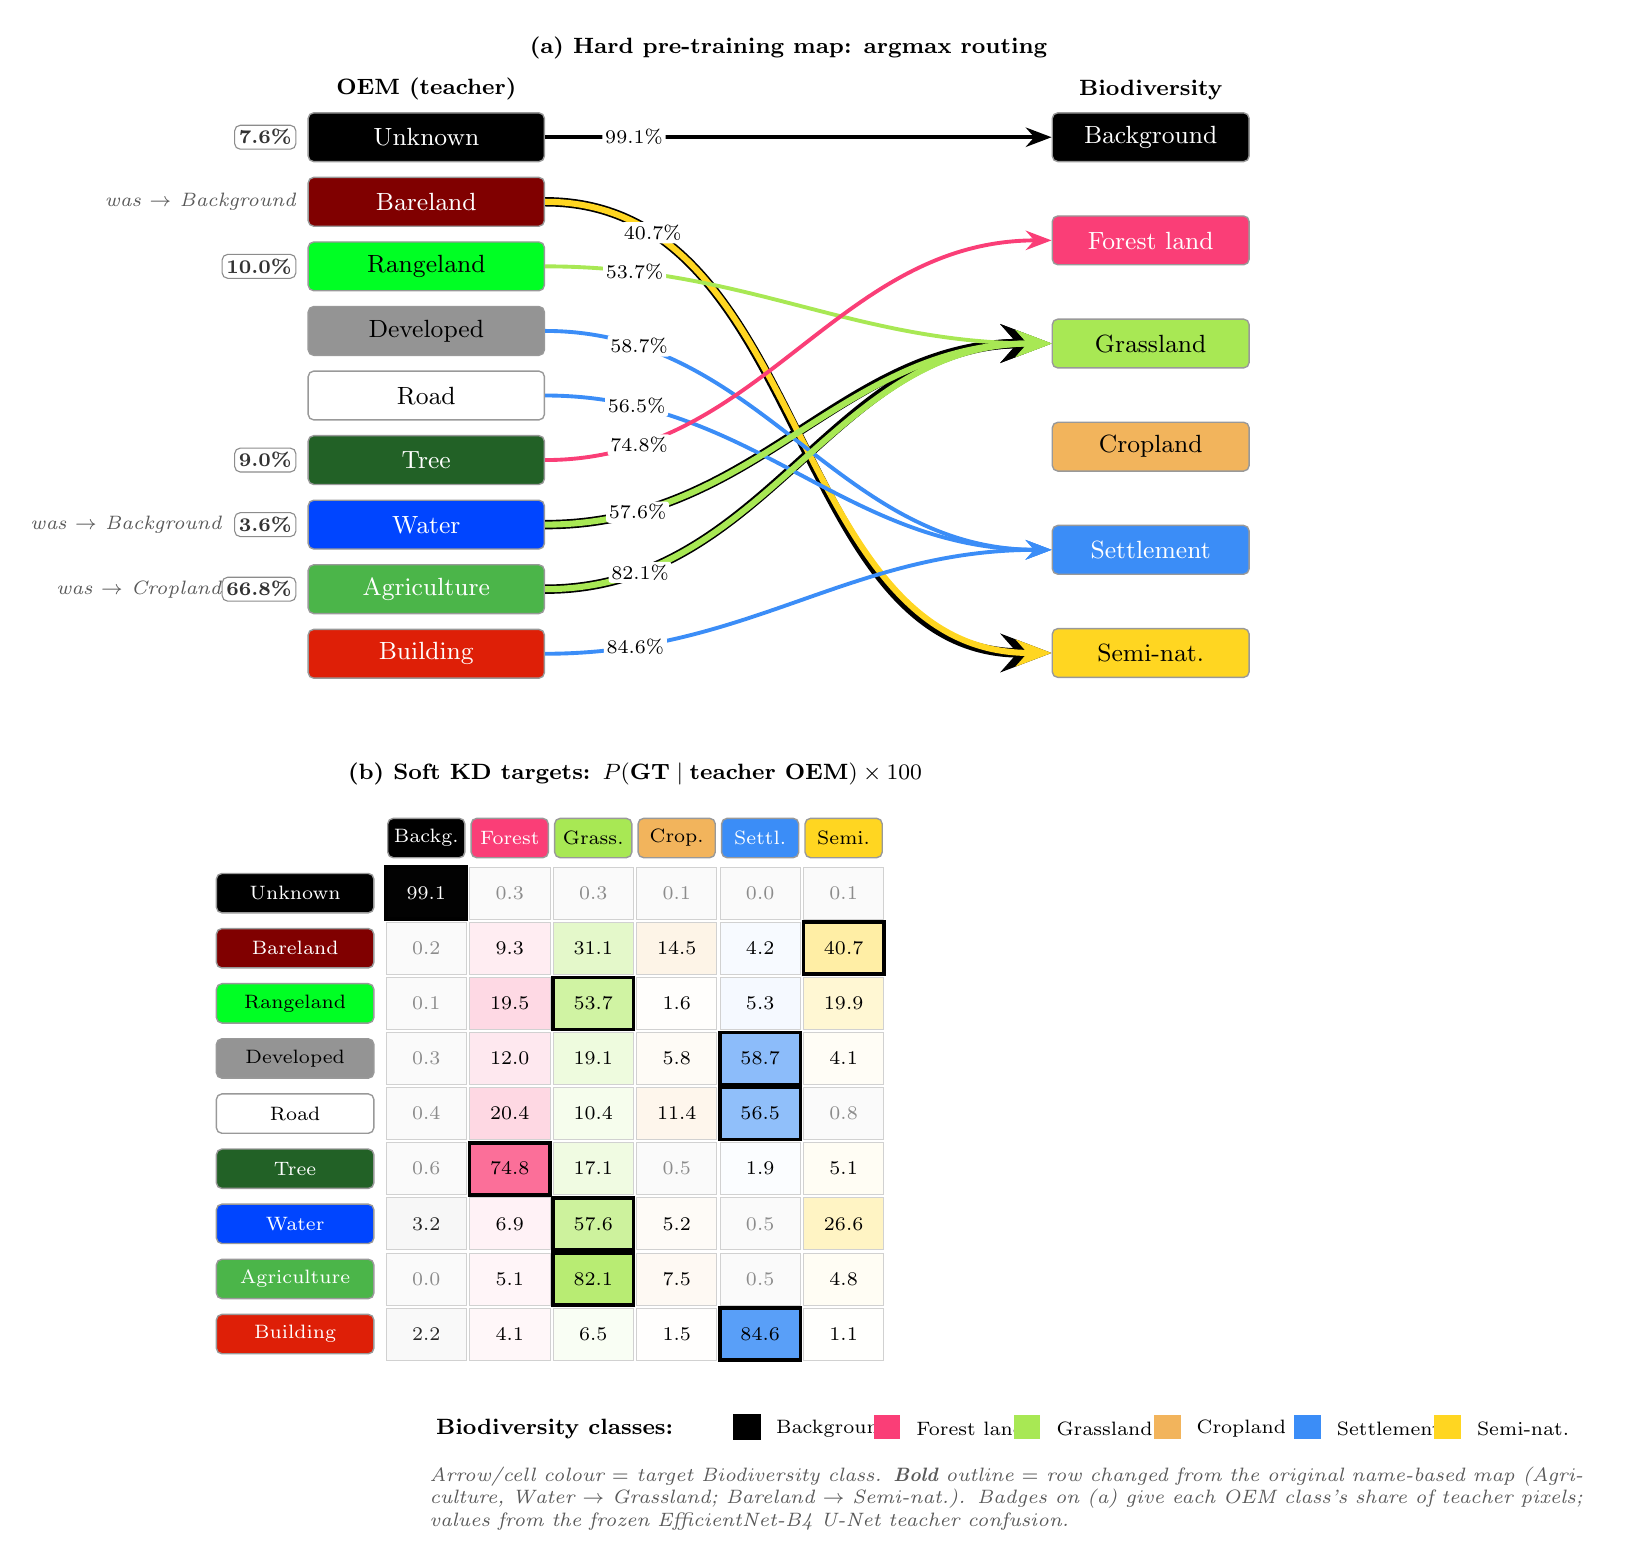
\begin{tikzpicture}[
  font=\small,
  >=Stealth,
  % OEM chip: fill = OEM colour, fixed size. White/black text set per chip.
  ochip/.style={
    rectangle, rounded corners=2pt, draw=black!40, line width=0.5pt,
    minimum width=3.0cm, minimum height=0.62cm, align=center, inner sep=2pt, font=\small
  },
  % student chip: fill = student colour.
  schip/.style={
    rectangle, rounded corners=2pt, draw=black!40, line width=0.5pt,
    minimum width=2.5cm, minimum height=0.62cm, align=center, inner sep=2pt, font=\small
  },
  % argmax arrow (normal): coloured the target student colour.
  arr/.style={->, line width=1.4pt},
  % argmax arrow for a CHANGED row: thicker + black halo behind.
  arrchg/.style={->, line width=2.2pt},
  conf/.style={fill=white, inner sep=1pt, font=\scriptsize, rounded corners=1pt},
  badge/.style={fill=white, draw=black!45, line width=0.4pt, rounded corners=2pt,
                inner sep=1.5pt, font=\scriptsize\bfseries, text=black!80},
  ann/.style={font=\scriptsize\itshape, text=black!65, inner sep=1pt},
  % Panel-B cell.
  cell/.style={rectangle, draw=black!18, line width=0.3pt,
               minimum width=1.02cm, minimum height=0.66cm, inner sep=0pt, font=\scriptsize},
  cellarg/.style={cell, draw=black, line width=1.3pt},
  hdr/.style={font=\footnotesize\bfseries, align=center},
]

% =====================================================================
% PANEL A — hard argmax (Sankey-style)
% =====================================================================
% OEM rows (top->bottom, OEM index order 0..8). y spacing 0.82cm.
\def\rowsep{0.82}
% (name, fill colour, white-text?, share-badge or empty)
% white-text chips: Unknown, Bareland, Tree, Water, Agriculture, Building, (Forest/Settlement on right)
\foreach \i/\nm/\col/\wt in {%
  0/Unknown/oUnknown/1,
  1/Bareland/oBare/1,
  2/Rangeland/oRange/0,
  3/Developed/oDev/0,
  4/Road/oRoad/0,
  5/Tree/oTree/1,
  6/Water/oWater/1,
  7/Agriculture/oAgri/1,
  8/Building/oBuild/1%
}{
  \pgfmathsetmacro{\yy}{-\i*\rowsep}
  \ifnum\wt=1
    \node[ochip, fill=\col, text=white] (oem\i) at (0,\yy) {\nm};
  \else
    \node[ochip, fill=\col, text=black] (oem\i) at (0,\yy) {\nm};
  \fi
}

% Teacher-pixel SHARE badges (HARD array; _gen_mapping_values.py), share > 3%.
%   Unknown 7.6, Rangeland 10.0, Tree 9.0, Water 3.6, Agriculture 66.8.
% Placed immediately LEFT of each chip, vertically centred on its OWN row, so the share is
% unambiguously tied to its OEM class (not the chip above) and never hits the arrow start (right side).
\node[badge, anchor=east] at ([xshift=-4pt]oem0.west) {7.6\%};
\node[badge, anchor=east] at ([xshift=-4pt]oem2.west) {10.0\%};
\node[badge, anchor=east] at ([xshift=-4pt]oem5.west) {9.0\%};
\node[badge, anchor=east] at ([xshift=-4pt]oem6.west) {3.6\%};
\node[badge, anchor=east, font=\scriptsize\bfseries] at ([xshift=-4pt]oem7.west) {66.8\%};

% --- "was -> ..." grey-italic annotations for the 3 changed rows, to the LEFT of the chip.
%     Bareland has no share badge (keep close); Water/Agriculture also carry a badge, so push
%     their annotation further left to clear it. ---
\node[ann, anchor=east] at ([xshift=-3pt]oem1.west) {was $\rightarrow$ Background};
\node[ann, anchor=east] at ([xshift=-1.05cm]oem6.west) {was $\rightarrow$ Background};
\node[ann, anchor=east] at ([xshift=-1.05cm]oem7.west) {was $\rightarrow$ Cropland};

% Student chips (right column). Wider horizontal channel (x=9.2) keeps the curves shallow.
% white-text: Background, Forest, Settlement. black-text: Grassland, Cropland, Seminatural.
\def\stx{9.2}
\foreach \j/\nm/\col/\wt/\yy in {%
  0/Background/cBack/1/0.0,
  1/{Forest land}/cForest/1/-1.31,
  2/Grassland/cGrass/0/-2.62,
  3/Cropland/cCrop/0/-3.93,
  4/Settlement/cSettle/1/-5.24,
  5/{Semi-nat.}/cSemi/0/-6.55%
}{
  \ifnum\wt=1
    \node[schip, fill=\col, text=white] (st\j) at (\stx,\yy) {\nm};
  \else
    \node[schip, fill=\col, text=black] (st\j) at (\stx,\yy) {\nm};
  \fi
}

% --- argmax arrows: OEM i -> student argmax, coloured the TARGET student colour. ---
% (oem, student-target, target-colour, conf%, changed?)
%   Unknown->Background 99.1 ; Bareland->Semi 40.7 CHG ; Rangeland->Grass 53.7 ;
%   Developed->Settle 58.7 ; Road->Settle 56.5 ; Tree->Forest 74.8 ;
%   Water->Grass 57.6 CHG ; Agriculture->Grass 82.1 CHG ; Building->Settle 84.6.
% Black halo first for the 3 changed rows, then the coloured arrow on top.
\foreach \oi/\sj in {1/5, 6/2, 7/2}{
  \draw[->, line width=3.4pt, black, rounded corners]
    (oem\oi.east) to[out=0,in=180] (st\sj.west);
}
% Confidence labels are anchored NEAR THE SOURCE (pos=0.16) so each sits beside its own OEM
% row and they fan out vertically instead of stacking at the convergence point.
\foreach \oi/\sj/\col/\cf/\chg in {%
  0/0/cBack/99.1/0,
  1/5/cSemi/40.7/1,
  2/2/cGrass/53.7/0,
  3/4/cSettle/58.7/0,
  4/4/cSettle/56.5/0,
  5/1/cForest/74.8/0,
  6/2/cGrass/57.6/1,
  7/2/cGrass/82.1/1,
  8/4/cSettle/84.6/0%
}{
  \ifnum\chg=1
    \draw[arrchg, \col, rounded corners] (oem\oi.east) to[out=0,in=180]
      node[conf, pos=0.16, text=black]{\cf\%} (st\sj.west);
  \else
    \draw[arr, \col] (oem\oi.east) to[out=0,in=180]
      node[conf, pos=0.16, text=black]{\cf\%} (st\sj.west);
  \fi
}

% Panel-A title
\node[hdr, anchor=south] at ($(oem0.north)!0.5!(st0.north)+(0,0.55)$)
  {(a) Hard pre-training map: argmax routing};
\node[font=\footnotesize\bfseries, anchor=south] at ([yshift=1pt]oem0.north) {OEM (teacher)};
\node[font=\footnotesize\bfseries, anchor=south] at ([yshift=1pt]st0.north) {Biodiversity};

% =====================================================================
% PANEL B — soft KD transition matrix (9x6 value-scaled heatmap)
% =====================================================================
% Anchor Panel B below Panel A.
\def\bx{0.0}            % left edge x of matrix body
\def\by{-9.6}          % top edge y of first data row
\def\cw{1.06}          % column step
\def\ch{0.70}          % row step

% Column headers (student chips, compact)
\foreach \j/\nm/\col/\wt in {%
  0/{Backg.}/cBack/1, 1/{Forest}/cForest/1, 2/{Grass.}/cGrass/0,
  3/{Crop.}/cCrop/0, 4/{Settl.}/cSettle/1, 5/{Semi.}/cSemi/0%
}{
  \pgfmathsetmacro{\cx}{\bx + \j*\cw}
  \ifnum\wt=1
    \node[schip, fill=\col, text=white, minimum width=0.98cm, minimum height=0.5cm, font=\scriptsize]
      at (\cx,{\by+\ch}) {\nm};
  \else
    \node[schip, fill=\col, text=black, minimum width=0.98cm, minimum height=0.5cm, font=\scriptsize]
      at (\cx,{\by+\ch}) {\nm};
  \fi
}

% Row headers (OEM chips, compact) + cells.
% Per row: argmax column index, and the 6 percentages (SOFT matrix x100; _gen_mapping_values.py).
\foreach \i/\nm/\rcol/\rwt/\arg/\va/\vb/\vc/\vd/\ve/\vf in {%
  0/Unknown/oUnknown/1/0/99.1/0.3/0.3/0.1/0.0/0.1,
  1/Bareland/oBare/1/5/0.2/9.3/31.1/14.5/4.2/40.7,
  2/Rangeland/oRange/0/2/0.1/19.5/53.7/1.6/5.3/19.9,
  3/Developed/oDev/0/4/0.3/12.0/19.1/5.8/58.7/4.1,
  4/Road/oRoad/0/4/0.4/20.4/10.4/11.4/56.5/0.8,
  5/Tree/oTree/1/1/0.6/74.8/17.1/0.5/1.9/5.1,
  6/Water/oWater/1/2/3.2/6.9/57.6/5.2/0.5/26.6,
  7/Agriculture/oAgri/1/2/0.0/5.1/82.1/7.5/0.5/4.8,
  8/Building/oBuild/1/4/2.2/4.1/6.5/1.5/84.6/1.1%
}{
  \pgfmathsetmacro{\ry}{\by - \i*\ch}
  \ifnum\rwt=1
    \node[ochip, fill=\rcol, text=white, minimum width=2.0cm, minimum height=0.5cm, anchor=east,
          font=\scriptsize] at ({\bx-0.62*\cw},\ry) {\nm};
  \else
    \node[ochip, fill=\rcol, text=black, minimum width=2.0cm, minimum height=0.5cm, anchor=east,
          font=\scriptsize] at ({\bx-0.62*\cw},\ry) {\nm};
  \fi
  % 6 cells; background = student-column colour scaled by value (fill=col!val).
  \foreach \j/\col/\val in {0/cBack/\va,1/cForest/\vb,2/cGrass/\vc,3/cCrop/\vd,4/cSettle/\ve,5/cSemi/\vf}{
    \pgfmathsetmacro{\cx}{\bx + \j*\cw}
    % blanked grey for <1% ; scaled colour otherwise ; bold border on argmax.
    \pgfmathparse{\val<1.0 ? 1 : 0}\edef\isblank{\pgfmathresult}
    % colour mix: cap at 90 for readability of dark student colours; Background(black) handled below.
    \pgfmathsetmacro{\mix}{min(\val,100)}
    \ifnum\j=0
      % Background column is black -> scale fill on black; pick text colour by fill darkness so
      % small-but->=1 values (Water 3.2, Building 2.2) are not rendered white-on-near-white.
      \ifnum\isblank=1
        \node[cell, fill=gray!4, text=black!45] (c\i\j) at (\cx,\ry) {\val};
      \else
        \pgfmathparse{\mix<40 ? 1 : 0}\edef\lightbg{\pgfmathresult}
        \ifnum\lightbg=1
          \node[cell, fill=black!\mix, text=black!85] (c\i\j) at (\cx,\ry) {\val};
        \else
          \node[cell, fill=black!\mix, text=white] (c\i\j) at (\cx,\ry) {\val};
        \fi
      \fi
    \else
      \ifnum\isblank=1
        \node[cell, fill=gray!4, text=black!45] (c\i\j) at (\cx,\ry) {\val};
      \else
        \node[cell, fill=\col!\mix] (c\i\j) at (\cx,\ry) {\val};
      \fi
    \fi
  }
  % bold border on argmax cell
  \pgfmathsetmacro{\acx}{\bx + \arg*\cw}
  \node[cellarg] at (\acx,\ry) {};
}

% Panel-B title
\node[hdr, anchor=south] at ({\bx+2.5*\cw},{\by+\ch+0.55})
  {(b) Soft KD targets: $P(\text{GT} \mid \text{teacher OEM}) \times 100$};

% =====================================================================
% SHARED LEGEND
% =====================================================================
\def\lgy{-16.4}
\node[font=\footnotesize\bfseries, anchor=west] at (\bx,\lgy) {Biodiversity classes:};
\foreach \k/\nm/\col/\edge in {%
  0/Background/cBack/1,
  1/{Forest land}/cForest/0,
  2/Grassland/cGrass/0,
  3/Cropland/cCrop/0,
  4/Settlement/cSettle/0,
  5/{Semi-nat.}/cSemi/0%
}{
  \pgfmathsetmacro{\lx}{\bx + 3.9 + \k*1.78}
  \ifnum\edge=1
    \fill[\col, draw=black, line width=0.5pt] (\lx,{\lgy-0.13}) rectangle ++(0.34,0.30);
  \else
    \fill[\col] (\lx,{\lgy-0.13}) rectangle ++(0.34,0.30);
  \fi
  \node[anchor=west, font=\scriptsize] at ({\lx+0.42},\lgy) {\nm};
}
\node[ann, anchor=north west, text width=15cm] at (\bx,{\lgy-0.45})
  {Arrow/cell colour $=$ target Biodiversity class. \textbf{Bold} outline $=$ row changed from the
   original name-based map (Agriculture, Water $\rightarrow$ Grassland; Bareland $\rightarrow$
   Semi-nat.). Badges on (a) give each OEM class's share of teacher pixels; values from the frozen
   EfficientNet-B4 U-Net teacher confusion.};

\end{tikzpicture}
\end{document}
